\documentclass{article}
\usepackage{amsmath, amsthm, amssymb, amsfonts}
\usepackage{thmtools}
\usepackage{graphicx}
\usepackage{setspace}
\usepackage{geometry}
\usepackage{float}
\usepackage{hyperref}
\usepackage[utf8]{inputenc}
\usepackage[english]{babel}
\usepackage{framed}
\usepackage[dvipsnames]{xcolor}
\usepackage{tcolorbox}
\usepackage{amsmath}
\usepackage{array}
\usepackage{tikz} 
\usepackage{multirow}
\usepackage{tcolorbox}
\usepackage{xcolor}

% Define a new color for the example box



\colorlet{LightGray}{White!90!Periwinkle}
\colorlet{LightOrange}{Orange!15}
\colorlet{LightGreen}{Green!15}

\newcommand{\HRule}[1]{\rule{\linewidth}{#1}}

\colorlet{LightGray}{black!10}
\colorlet{LightOrange}{orange!15}
\colorlet{LightGreen}{green!15}
\colorlet{LightBlue}{blue!15}
\colorlet{LightCyan}{cyan!15}



\declaretheoremstyle[name=Theorem,]{thmsty}
\declaretheorem[style=thmsty,numberwithin=section]{theorem}
\usepackage{tcolorbox} % Add missing package
\tcolorboxenvironment{theorem}{colback=LightGray}

\declaretheoremstyle[name=Definition,]{thmsty}
\declaretheorem[style=thmsty,numberwithin=section]{definition}
\tcolorboxenvironment{definition}{colback=LightBlue}

\declaretheoremstyle[name=Proposition,]{prosty}
\declaretheorem[style=prosty,numberlike=theorem]{proposition}
\tcolorboxenvironment{proposition}{colback=LightOrange}


\declaretheoremstyle[name=Example,]{prosty}
\declaretheorem[style=prosty,numberlike=theorem]{example}
\tcolorboxenvironment{example}{colback=LightOrange}

\declaretheoremstyle[name=Axiom,]{prcpsty}
\declaretheorem[style=prcpsty,numberlike=theorem]{axiom}
\tcolorboxenvironment{axiom}{colback=LightGreen}

\declaretheoremstyle[name=Lemma,]{prcpsty}
\declaretheorem[style=prcpsty,numberlike=theorem]{lemma}
\tcolorboxenvironment{lemma}{colback=LightCyan}





\setstretch{1.2}
\geometry{
    textheight=9in,
    textwidth=5.5in,
    top=1in,
    headheight=12pt,
    headsep=25pt,
    footskip=30pt
}

% ------------------------------------------------------------------------------

\begin{document}

% ------------------------------------------------------------------------------
% Cover Page and ToC
% ------------------------------------------------------------------------------

\title{ \normalsize \textsc{}
		\\ [2.0cm]
		\HRule{1.5pt} \\
		\LARGE \textbf{\uppercase{Stabilizers and Orbits}}
		\HRule{2.0pt} \\ [0.6cm] \LARGE{Cosets}
		}

\date{\today}
\author{\textbf{Author} \\ 
		Tom Jeong
        }

\maketitle
\newpage

\tableofcontents
\newpage

% ------------------------------------------------------------------------------
\section{Stabilizers}
From last class, $\sigma = (123)(56)  \in S_6$ \\ 
$H = <\sigma >  = \{\sigma, \sigma^2, \sigma^3, \sigma^4, \sigma^5, e\}$ 
and \\ $H \circlearrowright M_6 = \{1,2,3,4,5,6\}$ \\
The sets of orbit $M_6 / H = \{ \{1,2,3\}, \{4,5,6\} \}$ \\

The stablizer:
\begin{align*}
    H_{\{1\} } &= \{e, \sigma^3\} \\
    H_{\{4\} } &= H \\ 
    H_{\{5\} } &= \{\sigma^2, \sigma^4, e\} \\ 
    H_{\{5,6\} } &= \{h \in H | h \cdot \{5, 6\} = \{5, 6\} \} = H
\end{align*}
Ex: Let $H \leq G$ \\ 
THen\begin{align*}
    \alpha: H \times G &\to G \\ 
    \alpha(h, g) &= h \cdot g
\end{align*} is an action $H \circlearrowright G$ \\  the orbit $H \cdot g = \{hg | h \in H\}$
ie the right coset $Hg$ the set of orbit is $H \backslash G$   \\ 
ie the sest of right cosets 
fixed poitns $H_g = \{h \in H | hg = g\}$ \\ ther is no fixed points since $H \not = \{e\}$ \\ 
\subsection{examples}
ex. $GL_2(\mathbb{R}) \circlearrowright \mathbb{R}^2$ by \begin{align*}
    \alpha &= GL_2(\mathbb{R}) \times \mathbb{R}^2 \to \mathbb{R}^2 \\ 
    \alpha(A, v) &= A \cdot v
\end{align*}
\begin{align*}
    A \cdot (0,0 ) &= (0,0) \text{ } \forall A \in GL_2(\mathbb{R}) \\
    \text{ If } \vec{v} &\not = (0,0 ), \\ 
    & GL_2(\mathbb{R} ) \cdot \vec{v} = \mathbb{R}^2 \backslash \{(0,0)\}\\ 
    \text{ Let } S' &= \{\vec{v} \in \mathbb{R}^2 | ||\vec{v}|| = 1\} \\
 \end{align*} \\ 
 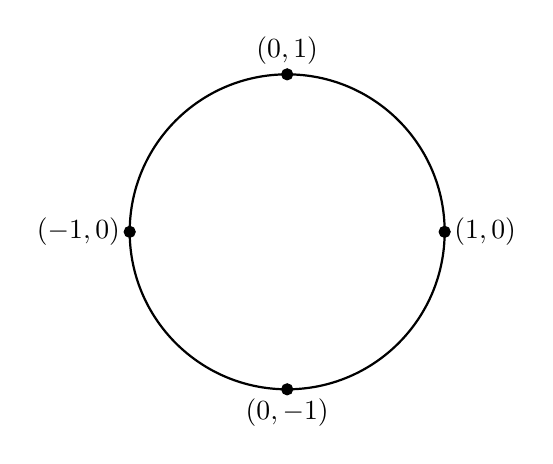
\begin{tikzpicture}
    % Draw the unit circle
    \draw[thick] (0,0) circle (2);
    
    % Label points on the circle
    \filldraw (2,0) circle (2pt) node[anchor=west] {$(1,0)$};
    \filldraw (-2,0) circle (2pt) node[anchor=east] {$(-1,0)$};
    \filldraw (0,2) circle (2pt) node[anchor=south] {$(0,1)$};
    \filldraw (0,-2) circle (2pt) node[anchor=north] {$(0,-1)$};
    
    % Arrows indicating stabilizer group action
    
    % Center point
    
    % Label for S'
    
\end{tikzpicture} \\ 
\underline{exercise}: stabilizer of S' is $O_2(\mathbb{R}) = \{A \in GL_2(\mathbb{R}) | A^T A = id\}$ \\
\underline{exercise} Let H be a subgroup of G not necessarily normal \\ 

Then Define 
\\ 
\begin{align*}
    \alpha:& G \times G / H \to G / H \\
    \alpha& (g, g'H) = (gg')H
\end{align*}
Tere is only one orbit since for any $g_1H$ and $g_2H$, $$\alpha(g_2g_{1}^{-1}, g_1H) = g_2H$$
The stabilizer of $H \in G/ H $ is $H \leq G$ since $\alpha(h,H) = hH = H$ for all $h \in H$ \\




%%%%%%%%%%%%%%%%%%%%%%%%%%%%%%%%%%%%%%%%%%%%%%%%%%%%%%%%%%%%%%%%%%%%%%%%%%%%%%%%%%%%%%%%%%%%
\begin{proposition}
    
    Let $\alpha: G \times S \to S$ be a group action. \begin{enumerate}
        \item let $X \subseteq S$ Then the stabilizer $G_X$ is a subsgroup of $G$ 
        \item The set $S$ is a union of $G$-ortbits. $$S = \bigcup_{s \in S} G \cdot s$$ where 
        $G \cdot s \not = G \cdot t \longrightarrow G \cdot s \cap G \cdot t = \emptyset$
        \item Orbit-stabilizer lemma: Let $x \in S$ then $$\tilde{f}: G/ G_X \to G \cdot x $$ given by $\tilde{f}(gG_x) = g \cdot x$ is a well-defined bijection map between the set of left osets of $G_X$ and the orbit of $x$ 
        
    \end{enumerate}
\end{proposition}

EX. 
\begin{example}
    \begin{align*}
        \sigma &= (123)(56) \in S_6 \\
        H &= <\sigma> \\ 
        H &\circlearrowright M_6 \\
    \end{align*}
    set of orbits $$M_6 / H =  \{ \{1,2,3\}, \{4\}, \{5,6\} \}$$
    with Stabilizer: \begin{align*}
        H_{1} & = \{e, \sigma^3\} \\
        H_{5} & = \{\sigma^2, \sigma^4, e\} \\
        H / H_{5} &= \{H_{5}, \sigma H_{5}\}\\ 
        \text{ Note that } & \sigma H_{5} = \{\sigma \sigma^2, \sigma \sigma^4, \sigma e\} = \{\sigma^3, \sigma^5, \sigma\} = H_{1}
    \end{align*} 
    with the bijection
    \begin{align*}
        \tilde{f}: H / H_{5} &\to \{5,6\} \\ 
        \tilde{f}(H_{5}) &= 5 \\
        \tilde{f}(\sigma H_{5}) &= 6
    \end{align*}
\end{example}
Now since we have seen the sample, we will show the proof of the proposition. \begin{proof}
    \leavevmode \\ 
    \begin{enumerate}
        \item Prove that $G_X$ is a subgroup $G_X = \{g \in G | gX = X \}$ \\(Identity) $e \in G_X$ (by definitino of group action) \\ 
            (Closure) If $g,h \in G_X$ then $(gh) \cdot X = g(h\cdot X) = gX = X$  \\ 
            (Inverse) If $g \in G_X$ then $g^{-1}X = g^{-1}(gX) = X$  since g is in the stabilizer\\
        \item We will define an equivalence relation: define $\alpha: G \times S \to S $ be a group action. LEt $s,t \in S $ Define $s \sim t$ if $\exists g \in G$ such that $g \cdot s = t$ \\
        \begin{lemma}
            This is an equivalence relation. \begin{proof} \leavevmode \\
                \begin{enumerate}
                    \item \underline{reflexive}: $e \in G$ and $e \cdot s = s$ forall $s\in S$ so $s \sim s$
                    \item \underline{symmetric}: suppose $s \sim t$ then $\exists g \in G $ such that $g \cdot s  = t$ \\ then $g^[-1] \cdot t = g^{-1} (gs) = e\cdot s = s$ so $t \sim s$
                    \item \underline{transitive}: suppose $s \sim t $ and $t \sim u$ then $\exists g, h \in G$ such that $g\cdot s = t$ and $h \cdot t = u$ \\ $hg\cdot s = ht = u$ so $s \sim u$
                     
                \end{enumerate}
                So $g$ orbits are eactly the equivalence classes of this relation. 
            \end{proof}
        \end{lemma}
        \item wts: $\tilde{f}: G / G_X \to G\cdot x$ with $\tilde{f}(gG_X) = g \cdot x$ is a well-defined bijection. \\ 
        Let $g_1, g_2 \in G$ suppose $g_2 G_x = g_2 G_X$. By Lemme 2.26 $$g_1G_X = g_2G_X \leftrightarrows g_1^{-1}g_2 \in G_X$$ we have that $g_1^{-1} g_2 \in G_x $ \\ liff $g_1^{-1}g_2 \cdot x = x$ \\ iff $g_1 \cdot x = g_2 \cdot x$ so $\tilde{f}$ is well-defined and injective  \\ Let $s \in G\cdot x$ Then $s = g\cdot x$ for some $g \in G$.. Hence $$\tilde{f}(gG_X) = g\cdot x$$ so $\tilde{f}$ is surjective 

    \end{enumerate}
\end{proof}

\begin{example}
    
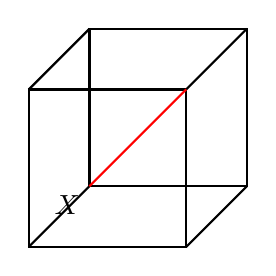
\begin{tikzpicture}[scale=2]
    % Draw cube
    \draw[thick] (0, 0, 0) -- (1, 0, 0) -- (1, 1, 0) -- (0, 1, 0) -- cycle; % bottom face
    \draw[thick] (0, 0, 1) -- (1, 0, 1) -- (1, 1, 1) -- (0, 1, 1) -- cycle; % top face
    \draw[thick] (0, 0, 0) -- (0, 0, 1); % left edge
    \draw[thick] (1, 0, 0) -- (1, 0, 1); % right edge
    \draw[thick] (1, 1, 0) -- (1, 1, 1); % back edge
    \draw[thick] (0, 1, 0) -- (0, 1, 1); % front edge

    % Label vertex X outside the cube
    \node at (0, 0, 0) [below left] {$X$};

    % Draw red axis from X to the opposite vertex
    \draw[red, thick] (0, 0, 0) -- (1, 1, 1);
\end{tikzpicture} x should be on top righr coerner ngl 
    Let $G = \{\text{ group of symmetries of a cube}\}$. WHat is the order of G? \\ Let $x$ be a vertex, $|G\cdot x|= 8$ since the orbit of x is the number of vertices of the cube. 
    
     Stabilizer $|G_X| = 3$ which is the identity, rotation by $\frac{2\pi}{3}, \frac{4\pi}{3}$ \\about the red axis
     By LaGranges Theorem $|G| = |G / G_X| \cdot |G_X| = 8 \cdot 3 = 24$by Previous proposition $|G / G_X |  = |G \cdot X| = 8$ SO we have $|G| = 24$
\end{example}
\underline{Corollary} (2.10.7) Let $G \times S \to S$ be a group action where $S$ is a finnite set \\ Then 
$$|S| = |S^G| + \sum_{x} |G / G_X | $$ where $S^G$ are the fixed points. where the summation is done by picking out an element x from eah orbit with more than one element.
\begin{proof}
    \leavevmode \\
    BY 2) of the previous proposition $|S| = \sum_{G\cdot X \in S/ G} |G \cdot x| = $ \[
| S^G | \text{ (orbits containing a single element) } + \sum_{x} | G / G_X | \text{ (by part 3 of proposition) }
\]


\end{proof}

\begin{lemma}[ Burnside's Lemma (2.10.8)] \leavevmode \\ 
    Cauchy -Frobenius Lemma. 
    Let $G \times S \to S$ be a group action where $S$ is a finite set and $G$ is a finite group. Then the number of orbits is equal to the average number of fixed points of elements of $G$.
    $$|S / G| = \cfrac{\sum_{g\in G} |S^g|}{|G|}  $$
    and where $S^g = \{x\in S | gx = x\}$
\end{lemma}
\end{document}
 